\documentclass[9pt,twocolumn,twoside]{styles/osajnl}
\usepackage{fancyvrb}
\journal{i524} 

\title{Analysis of H-1B Temporary Employment-Based in Data Science Profession}


\author[1,*]{Jimmy Ardiansyah}

\affil[1]{School of Informatics and Computing, Bloomington, IN 47408, U.S.A.}


\affil[*]{jardians@indiana.edu - S17-IR-2002}

\dates{Project Proposal, \today}


\ociscodes{}

\ociscodes{Apach, Hadoop, H1B, Data Science}

% replace this with your url in github/gitlab
\doi{\url{https://github.com/jardians/sp17-i524/blob/master/project/S17-IR-2002/report/report.pdf}}
 
\begin{abstract}
This project aims to  analyze The H-1B  temporary employment-based visa for Data Science related jobs in the United States. We are trying to answer the number of questions related to Data Science related jobs in America’s workforce based on H-1B visa.
\newline  
\newline  
\end{abstract} 

   
\setboolean{displaycopyright}{true} 

\begin{document}

\maketitle

\section{Introduction}
Every day tech industry executive bemoan the lack of data scientists—the people who theoretically know how to look at the data your company generates, and delve into it to derive the all-important insights we keep hearing about. It’s no secret that there’s a shortage of data scientists in America’s workforce. Many companies look to hire overseas to help ease the domestic talent shortfall (in fact, one in three data scientists are born outside the U.S.) so understanding the ins and outs of visas is rapidly becoming a business necessity  ~\cite{www-hbr}. To accomplish the goals, I would like to answer question
like the following:

\begin{itemize}
  \item What is the number of petitions with Data Engineer or Scientist jobs title increasing over time?
  \item Which part of the US has the most Data Engineer or Scientist  jobs?
  \item what year petitions with Data Engineer or Scientist jobs granted the most between 2011 to 2016?
  \item  Which employers file the most petitions with Data Engineer or Scientist jobs title each year?
\end{itemize}


\section{Plan}
Following table gives a breakdown of tasks in order to complete the project. Assuming week1 starts after submission of the proposal. These work items are high level breakdown on the tasks and may changes if needed.

\begin{figure}[H]
 \centering
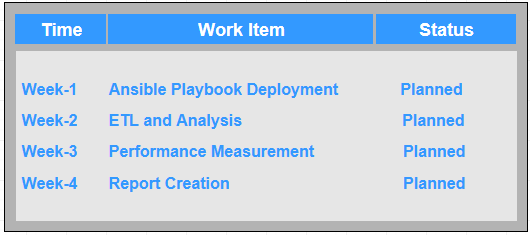
\includegraphics[scale=0.6]{images/image11}
\caption{Planned Schedule}
\end{figure}

\section{Design}

I break the high-level design of the technologies used into 3 main sectios-- storagee, ingestion, processing and analyzing. 

\begin{itemize}
  \item Storage refers to decision around the storage system such as HDFS or HBase
  \item Ingestion refers to getting data from source and loading it into Hadoop for processing.
  \item Analyzing refers to running various analytical queries on processed dataset to find answer and insight to the questions presented. 
\end{itemize}


\begin{figure}[H]
 \centering
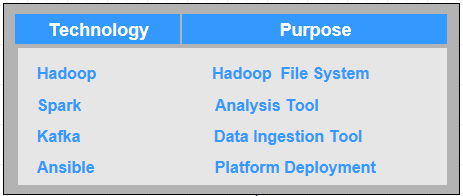
\includegraphics[scale=0.6]{images/image10}
\caption{Planned Technologies Deployment ~\cite{wiki-ansible} ~\cite{www-kafka} ~\cite{www-spark} ~\cite{wiki-hadoop}}
\end{figure}


In the design implementation, We will use HDFS ~\cite{wiki-hadoop}
 to store data, Kafka  ~\cite{www-kafka} for ingesting dataset from Kaggle.com ~\cite{www-kaggle} into Hadoop.  We will user Spark  ~\cite{www-spark} for processing and analyzing. 

\begin{figure}[H]
 \centering
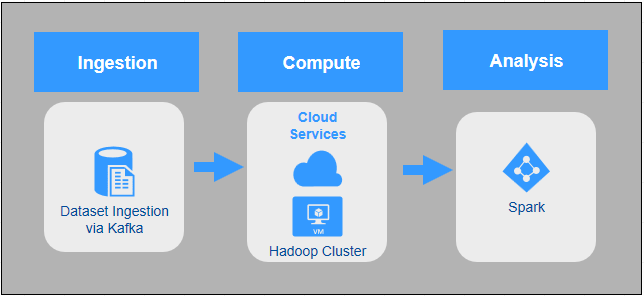
\includegraphics[scale=0.5]{images/image9}
\caption{Design Overview  ~\cite{www-kafka} ~\cite{www-spark} ~\cite{wiki-hadoop}}
\end{figure}


\section{Dataset Metadata Description}

The columns included in the dataset download from Kaggle ~\cite{www-kaggle} site  are followed  : 

\begin{itemize}
 \item  \verb|CASE_STATUS|: Status associated with the last significant event or decision.
 \item \verb|EMPLOYER_NAME|: Name of employer submitting labor condition application.
 \item  \verb|SOC_NAME|: the occupational code associated with the job being requested for temporary labor condition, as classified by the Standard Occupational Classification (SOC) System.
 \item  \verb|JOB_TITLE|: Title of the job
 \item  \verb|FULL_TIME_POSITION|: Y = Full Time Position; N = Part Time Position
 \item  \verb|PREVAILING_WAGE|: Prevailing Wage for the job being requested for temporary labor condition. The wage is listed at annual scale in USD. The prevailing wage for a job position is defined as the average wage paid to similarly employed workers in the requested occupation in the area of intended employment. The prevailing wage is based on the employer’s minimum requirements for the position. 
 YEAR: Year in which the H-1B visa petition was filed
 \item  WORKSITE: City and State information of the foreign worker's intended area of employment
 \item  LON: longitude of the Worksite
 \item  LAT: latitude of the Worksite
\end{itemize}

\section{Deployment}
Solution will be deployed using Ansible \cite{wiki-ansible} playbook. Automated deployment should happen on two or more nodes cluster. Deployment script should install all necessary software along with the project code to the cluster nodes.

\section{Benchmarking}
We will access the performance of the Hadoop/Spark clusters deployed on difference usage, storage size and IO througput. 

\section{Result}
Result of data analysis and benchmarking will be showcased in this section. 

\section{Conclusion}

Using this H-1B Visa Petitions 2011-2016 data from Kaggle,  we should be able build statiscal report regarding to Data Science Jobs related. 

\section{Acknowledgement}

This work was done as part of the course "I524: Big Data and Open Source Software Projects" at Indiana University during Spring 2017. We acknowledge our Professor Gregor Von Laszewski and all Associate Instructors for helping us and guiding us throughout this project.


% Bibliography

\bibliography{references}
\end{document}

